%%% LaTeX Template: Article/Thesis/etc. with colored headings and special fonts
%%%
%%% Source: http://www.howtotex.com/
%%% Feel free to distribute this template, but please keep to referal to http://www.howtotex.com/ here.
%%% February 2011
%%%
%%% Modified January 2016 by CDM

%%%  Preamble
\documentclass[11pt,letterpaper]{article}
\usepackage[margin=1.0in]{geometry}
\usepackage[T1]{fontenc}
\usepackage[bitstream-charter]{mathdesign}
\usepackage[latin1]{inputenc}					
\usepackage{amsmath}						
\usepackage{xcolor}
\usepackage{cite}
\usepackage{hyphenat}
\usepackage{graphicx}
\usepackage{float}
\usepackage{subfigure}
\usepackage{sectsty}
\usepackage[compact]{titlesec} 
\usepackage[tablegrid]{vhistory}
\usepackage{pbox}
\allsectionsfont{\color{accentcolor}\scshape\selectfont}

%%% Definitions
\definecolor{accentcolor}{rgb}{0.0,0.0,0.5} 
\newcommand{\teamname}{Team Name}
\newcommand{\productname}{Product Name}
\newcommand{\coursename}{CSE 4317: Senior Design II}
\newcommand{\semester}{Spring 2016}
\newcommand{\docname}{Detailed Design Specification}
\newcommand{\department}{Department of Computer Science \& Engineering}
\newcommand{\university}{The University of Texas at Arlington}
\newcommand{\authors}{Alan Turing \\ Grace Hopper \\ John Von Neumann \\ Ada Lovelace \\ Charles Babbage}

%%% Headers and footers
\usepackage{fancyhdr}
	\pagestyle{fancy}						% Enabling the custom headers/footers
\usepackage{lastpage}	
	% Header (empty)
	\lhead{}
	\chead{}
	\rhead{}
	% Footer
	\lfoot{\footnotesize \teamname \ - \semester}
	\cfoot{}
	\rfoot{\footnotesize page \thepage\ of \pageref{LastPage}}	% "Page 1 of 2"
	\renewcommand{\headrulewidth}{0.0pt}
	\renewcommand{\footrulewidth}{0.4pt}

%%% Change the abstract environment
\usepackage[runin]{abstract}			% runin option for a run-in title
%\setlength\absleftindent{30pt}			% left margin
%\setlength\absrightindent{30pt}		% right margin
\abslabeldelim{\quad}	
\setlength{\abstitleskip}{-10pt}
\renewcommand{\abstractname}{}
\renewcommand{\abstracttextfont}{\color{accentcolor} \small \slshape}	% slanted text

%%% Start of the document
\begin{document}

%%% Cover sheet
{\centering \huge \color{accentcolor} \sc \textbf{\department \\ \university} \par}
\vspace{1 in}
{\centering \huge \color{accentcolor} \sc \textbf{\docname \\ \coursename \\ \semester} \par}
\vspace{0.5 in}
\begin{figure}[h!]
	\centering
   	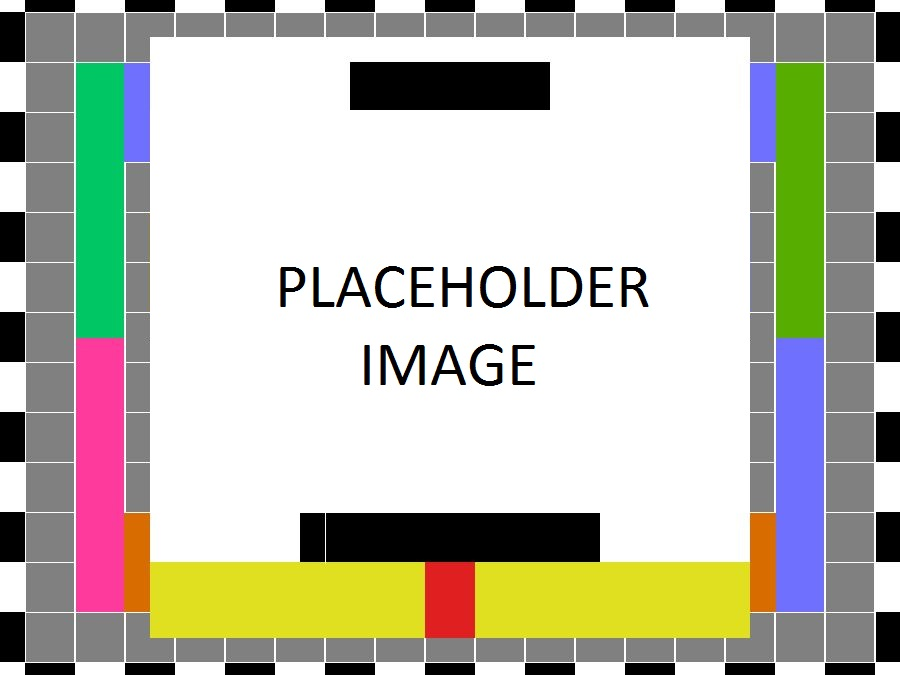
\includegraphics[width=0.60\textwidth]{images/test_image}
\end{figure}
\vspace{0.5 in}
{\centering \huge \color{accentcolor} \sc \textbf{\teamname \\ \productname} \par}
\vspace{0.5 in}
{\centering \large \sc \textbf{\authors} \par}
\newpage


%\vspace{1 in}
%\centerline{January 13th, 2012}
%\newpage

%%% Revision History
\begin{versionhistory}
  	\vhEntry{0.1}{1.01.2016}{GH}{document creation}
  	\vhEntry{0.2}{1.05.2016}{AT|GH}{complete draft}
  	\vhEntry{0.3}{1.12.2016}{AT|GH}{release candidate 1}
  	\vhEntry{1.0}{1.20.2016}{AT|GH|CB}{official release}
  	\vhEntry{1.1}{1.31.2016}{AL}{added design review requests}
\end{versionhistory}
\newpage

%%% Table of contents
\setcounter{tocdepth}{2}
\tableofcontents
\newpage

%%% List of figures and tables (optional)
\listoffigures
\listoftables
\newpage

%%% Document sections
\section{Introduction}
Your introduction should provide a brief overview of the product concept and a reference to the requirement specification and architectural design documents in 1 or 2 paragraphs. The purpose is to provide the reader with the location of relevant background material that lead to the design details presented in this document.

\section{System Overview}
The Brew System layer is the core of the Back Burner Brew. The goal of the project is to automate the brewing process, and although the system itself is very simple, the steps required to brew a proper beer is time consuming and requires a large amount of attention from the brewer. The user interface layer will ask the brewer to enter their desired temperature and time for each step of the brewing process. The analog and digital components will send data to the digital components. This data will contain the temperatures of the Hot Liqour Tank (HLT) and the mash tun, once the data is receieved by the digital components, the Web server layer will store that data into a cloud database and that data will be used to determine when a heating element or pump will turn on.
\begin{figure}[H]
	\centering
	\graphicspath{.\images}
	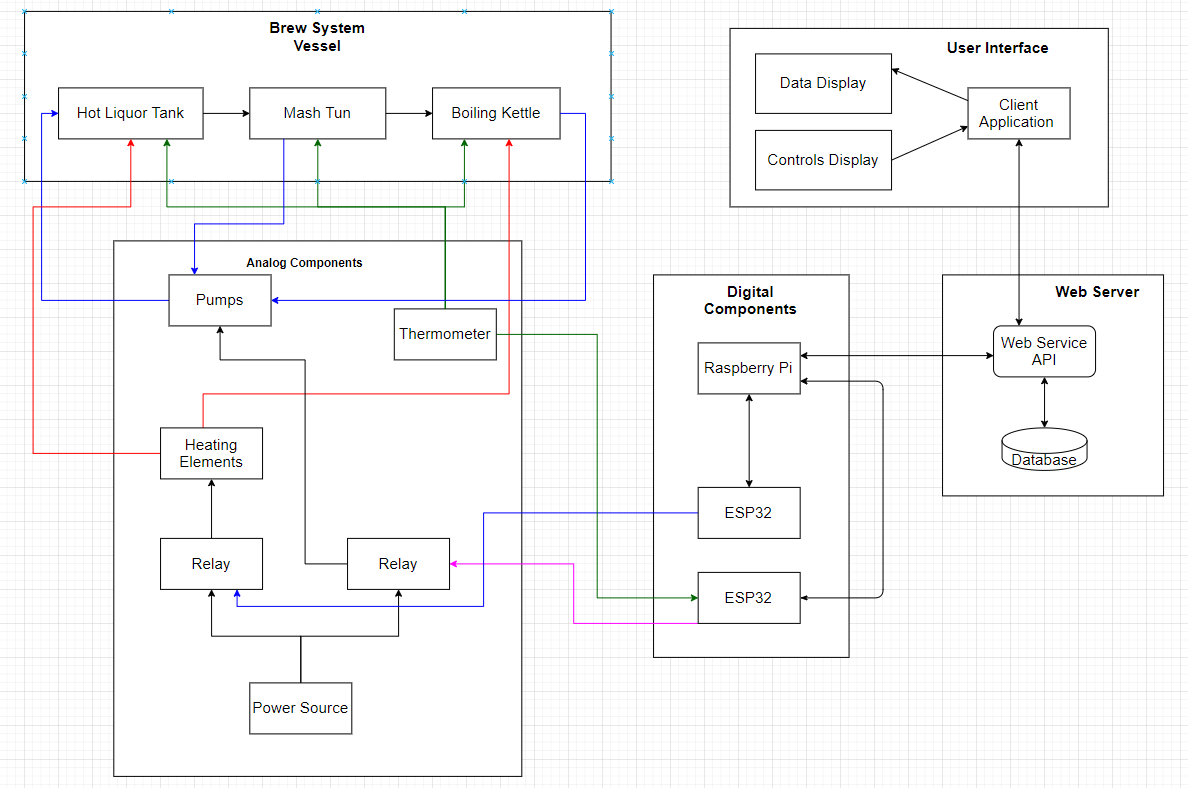
\includegraphics[scale=0.5]{images/sys_overview.PNG}
	\caption{System Overview}
\end{figure}
\newpage
%\section{Subsystem Definitions \& Data Flow}
%This section breaks down your layer abstraction to another level of detail. Here you grapically represent the logical subsytems that compose each layer and show the interactions/interfaces between those subsystems. A subsystem can be thought of as a programming unit that implements one of the major functions of the layer. It, therefore, has data elements that serve as source/sinks for other subsystems. The logical data elements that flow between subsystems need to be explicitly defined at this point, beginning with a data flow-like diagram based on the block diagram.

\begin{figure}[h!]
	\centering
 	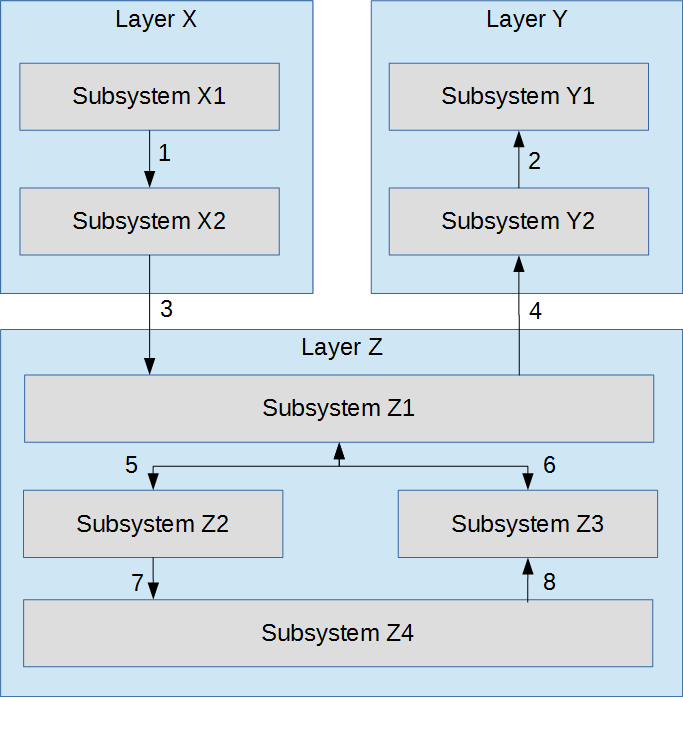
\includegraphics[width=\textwidth]{images/data_flow}
 \caption{A simple data flow diagram}
\end{figure}

\newpage
\section{X Layer Subsystems}
In this section, the layer is described in terms of the hardware and software design. Specific implementation details, such as hardware components, programming languages, software dependencies, operating systems, etc. should be discussed. Any unnecessary items can be ommitted (for example, a pure software module without any specific hardware should not include a hardware subsection). The organization, titles, and content of the sections below can be modified as necessary for the project.

\subsection{Layer Hardware}
A description of any involved hardware components for the layer. For example, if each subsystem is a software process running on an embedded computer, discuss the specifics of that device here. Do not list a hardware component that only exists at the subsystem level (include it in the following sections).

\subsection{Layer Operating System}
A description of any operating systems required by the layer.

\subsection{Layer Software Dependencies}
A description of any software dependencies (libraries, frameworks, etc) required by the layer.

\subsection{Subsystem 1}
Descibe at a high level the purpose and basic design of this subsystem. Is it a piece of hardware, a class, a web service, or something else? Note that each of the subsystem items below are meant to be specific to that subystem and not a repeat of anything discussed above for the overall layer.

\begin{figure}[h!]
	\centering
 	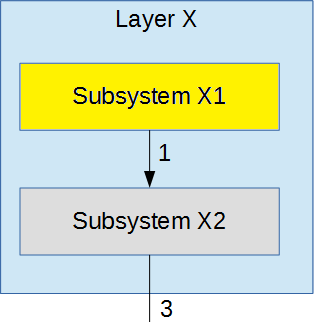
\includegraphics[width=0.60\textwidth]{images/subsystem}
 \caption{Example subsystem description diagram}
\end{figure}

\subsubsection{Subsystem Hardware}
A description of any involved hardware components for the subsystem.

\subsubsection{Subsystem Operating System}
A description of any operating systems required by the subsystem.

\subsubsection{Subsystem Software Dependencies}
A description of any software dependencies (libraries, frameworks, design software for mechanical parts or circuits, etc) required by the subsystem.

\subsubsection{Subsystem Programming Languages}
A description of any programming languages used by the subsystem.

\subsubsection{Subsystem Data Structures}
A description of any classes or other data structures that are worth discussing for the subsystem. For example, data being transmitted from a microcontroller to a PC via USB should be first be assembled into packets. What is the structure of the packets?

\subsubsection{Subsystem Data Processing}
A description of any algorithms or processing strategies that are worth discussing for the subsystem. If you are implementing a well-known algorithm, list it. If it is something unique to this project, discuss it in greater detail.



\newpage
\section{Y Layer Subsystems}
In this section, the layer is described in terms of the hardware and software design. Specific implementation details, such as hardware components, programming languages, software dependencies, operating systems, etc. should be discussed. Any unnecessary items can be ommitted (for example, a pure software module without any specific hardware should not include a hardware subsection). The organization, titles, and content of the sections below can be modified as necessary for the project.

\subsection{Layer Hardware}
A description of any involved hardware components for the layer. For example, if each subsystem is a software process running on an embedded computer, discuss the specifics of that device here. Do not list a hardware component that only exists at the subsystem level (include it in the following sections).

\subsection{Layer Operating System}
A description of any operating systems required by the layer.

\subsection{Layer Software Dependencies}
A description of any software dependencies (libraries, frameworks, etc) required by the layer.

\subsection{Subsystem 1}
Descibe at a high level the purpose and basic design of this subsystem. Is it a piece of hardware, a class, a web service, or something else? Note that each of the subsystem items below are meant to be specific to that subystem and not a repeat of anything discussed above for the overall layer.

\begin{figure}[h!]
	\centering
 	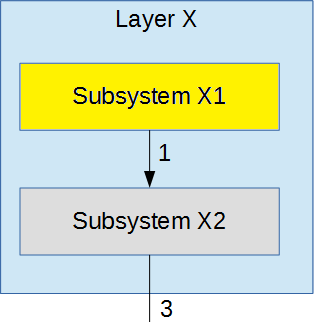
\includegraphics[width=0.60\textwidth]{images/subsystem}
 \caption{Example subsystem description diagram}
\end{figure}

\subsubsection{Subsystem Hardware}
A description of any involved hardware components for the subsystem.

\subsubsection{Subsystem Operating System}
A description of any operating systems required by the subsystem.

\subsubsection{Subsystem Software Dependencies}
A description of any software dependencies (libraries, frameworks, design software for mechanical parts or circuits, etc) required by the subsystem.

\subsubsection{Subsystem Programming Languages}
A description of any programming languages used by the subsystem.

\subsubsection{Subsystem Data Structures}
A description of any classes or other data structures that are worth discussing for the subsystem. For example, data being transmitted from a microcontroller to a PC via USB should be first be assembled into packets. What is the structure of the packets?

\subsubsection{Subsystem Data Processing}
A description of any algorithms or processing strategies that are worth discussing for the subsystem. If you are implementing a well-known algorithm, list it. If it is something unique to this project, discuss it in greater detail.



\newpage
\section{Digital Components Layer Subsystems}
The digital components layer will consist of 4 devices. The first is a Raspberry
PI. This will act as the main computer of the system. It will the majority of
the data both from the server, the UI, and the microcontrollers. The other 3
components will all be ESP32 microcontrollers, but they will each serve a
different purpose. An ESP32 will receive information from a thermometer sensor
and relay it to the heat control ESP32. Based on what the temperature is, the
heat control ESP32 will trigger the relay to activate or deactivate the heating
element. The final ESP32 will be used to trigger the relay to turn on the pump
based on what the message broker instructs it to do.   

\begin{figure}[h!]
	\centering
 	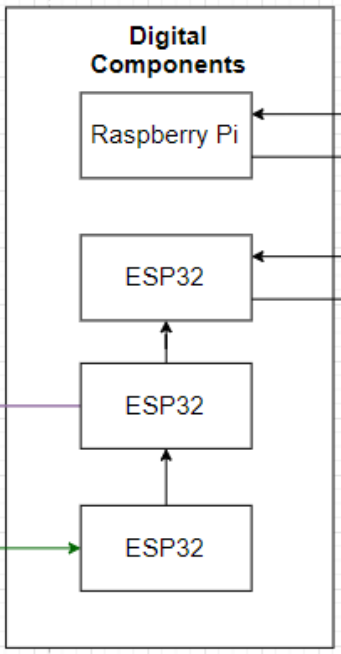
\includegraphics[width=0.30\textwidth]{images/digital_components.png}
  \caption{Digital Components Subsystem}
\end{figure}

\subsection{Digital Components Layer Hardware}
The hardware used in the digital components subsystem will made up of two
different types of electronics. The computer that acts as the arbiter of tasks
will be a Raspberry Pi 3b+. The microcontrollers used are ESP32s. 

\subsection{Digital Components Layer Operating System}
The Raspberry Pi 3b+ will run Raspbian OS. There will not be an operating system
on the microcontrollers. 

\subsection{Raspberry Pi Subsystem}
The Raspberry PI will host the web server and the MQTT client. The RBP will
receive information from the web server about what the user inputed via the UI.
It will then take that information and relay it to the microcontrollers using
the MQTT protocol. The RBP will then receive sensor data from the
microcontrollers through MQTT messages and send store the information in the web
server. 

\subsubsection{Subsystem Hardware}
The hardware involved in this layer will consist only of a Raspberry Pi 3b+.

\subsubsection{Subsystem Operating System}
The operating system used will be Raspbian OS.

\subsubsection{Subsystem Software Dependencies}
This subsystem will use the Mosquitto MQTT Message Broker. 

\subsubsection{Subsystem Programming Languages}
This subsystem will at the most use a scripting language such as BASH. 

\subsection{Temperature Sensor Subsystem}
The microcontroller will await messages from the message broker. The message
broker will recieve information from the thermometer ESP32. If the temperature
is too low, the message broker will send a message to this microcontroller to
trigger the relay and allow power to flow to the heating element. If the
temperature gets too high on the heating element, the message broker will tell
this microcontroller to deactivate the heating element.

\subsubsection{Subsystem Hardware}
The hardware involved in this layer will consist of a microcontroller ESP32 and a temperature
sensor MAX6675. 

\subsubsection{Subsystem Operating System}
None will be used for this subsystem.

\subsubsection{Subsystem Software Dependencies}
Arduino libraries will be used for the temperature sensor. 

\subsubsection{Subsystem Programming Languages}
C++ will be used to program the ESP32.

\subsubsection{Subsystem Data Structures}
The ESP32 will read data from the temperature sensor, and send it to the
Raspberry Pi for a decision to be made. The data will be passed via the MQTT protocol.

\subsection{Heat Control Subsystem}
The microcontroller will await messages from the message broker. The message
broker will recieve information from the thermometer ESP32. If the temperature
is too low, the message broker will send a message to this microcontroller to
trigger the relay and allow power to flow to the heating element. If the
temperature gets too high on the heating element, the message broker will tell
this microcontroller to deactivate the heating element.

\subsubsection{Subsystem Hardware}
The hardware involved will be an ESP32 and a 120V heating element. 

\subsubsection{Subsystem Operating System}
None will be used for this subsystem.

\subsubsection{Subsystem Software Dependencies}
Arduino MQTT libraries for the ESP32.

\subsubsection{Subsystem Programming Languages}
C++ will be used to program the ESP32.

\subsubsection{Subsystem Data Structures}
Commands will be sent to the ESP32 via MQTT messages. 

\subsection{Pump Control Subsystem}
This microcontroller will await messages from the message broker. When the
message broker sends it the message to turn on the pump, the microcontroller
will trigger the relay to allow power to go to the pump. When the message broker
sends the message to turn off the pump, the microcontroller will cease sending
power to the relay, causing it to close, and power will not be supplied to the
pump.

\subsubsection{Subsystem Hardware}
The hardware for this subsystem will consist of a single ESP32.

\subsubsection{Subsystem Operating System}
None will be used for this subsystem. 

\subsubsection{Subsystem Software Dependencies}
Arduino MQTT libraries for the ESP32.

\subsubsection{Subsystem Programming Languages}
C++ will be used to program the ESP32.

\subsubsection{Subsystem Data Structures}
Commands will be sent to the ESP32 via MQTT messages. 

\newpage
\section{Web Service Layer Subsystems}
In this section, the layer is described in terms of the hardware and software design. Specific implementation details, such as hardware components, programming languages, software dependencies, operating systems, etc. should be discussed. Any unnecessary items can be ommitted (for example, a pure software module without any specific hardware should not include a hardware subsection). The organization, titles, and content of the sections below can be modified as necessary for the project.

\subsection{Layer Hardware}
A description of any involved hardware components for the layer. For example, if each subsystem is a software process running on an embedded computer, discuss the specifics of that device here. Do not list a hardware component that only exists at the subsystem level (include it in the following sections).

\subsection{Layer Operating System}
A description of any operating systems required by the layer.

\subsection{Layer Software Dependencies}
A description of any software dependencies (libraries, frameworks, etc) required by the layer.

\subsection{Subsystem 1}
Descibe at a high level the purpose and basic design of this subsystem. Is it a piece of hardware, a class, a web service, or something else? Note that each of the subsystem items below are meant to be specific to that subystem and not a repeat of anything discussed above for the overall layer.

\begin{figure}[h!]
	\centering
 	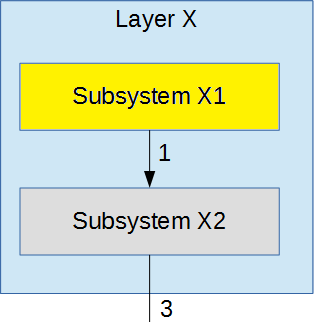
\includegraphics[width=0.60\textwidth]{images/subsystem}
 \caption{Example subsystem description diagram}
\end{figure}

\subsubsection{Subsystem Hardware}
A description of any involved hardware components for the subsystem.

\subsubsection{Subsystem Operating System}
A description of any operating systems required by the subsystem.

\subsubsection{Subsystem Software Dependencies}
A description of any software dependencies (libraries, frameworks, design software for mechanical parts or circuits, etc) required by the subsystem.

\subsubsection{Subsystem Programming Languages}
A description of any programming languages used by the subsystem.

\subsubsection{Subsystem Data Structures}
A description of any classes or other data structures that are worth discussing for the subsystem. For example, data being transmitted from a microcontroller to a PC via USB should be first be assembled into packets. What is the structure of the packets?

\subsubsection{Subsystem Data Processing}
A description of any algorithms or processing strategies that are worth discussing for the subsystem. If you are implementing a well-known algorithm, list it. If it is something unique to this project, discuss it in greater detail.



\newpage
\section{User Interface Layer Subsystems}
\subsection{User Interface}
The website used to control the system will be compatible with major web browsers and will be connected to a database and with the brewing system. Website is verified to work on Chrome for Windows 10, version 91.0.4472.124, and Chrome for MacOS Big Sur, version 91.0.4472.124

\subsection{Layer Operating System}
Website available on Windows 10 version 21H1 and MacOS Big Sur version 11.4

\subsection{Layer Software Dependencies}
The user interface components will depend on Mulesoft's Mule software, version 4.3.0

\subsection{Website}
The website provided to the user will have multiple responsabilities. First, it will display real-time information relevant to the user about the current brew. The website will also display a controls section for the user to interact with the brewing system. The information send to and from the website will be sent to the servers and then to the brewing system utilizing the above mentioned Mulesoft software.

\subsubsection{Subsystem Operating System}
No specific operating system required.

\subsubsection{Subsystem Software Dependencies}
The website and UI will utilize the React JS library

\subsubsection{Subsystem Programming Languages}
JavaScript will be used for creating the website.

\newpage
\section{Appendix A}
Include any additional documents (CAD design, circuit schematics, etc) as an appendix as necessary.
\newpage

%%% References
\bibliographystyle{plain}
\bibliographystyle{reference/IEEEtran_custom}
\bibliography{reference/refs}{}

\end{document}
